% Generated by pysimcount.figleader -- do not edit; regenerate instead.
% figure: main-cnot-all-formulas -- source curves (no error bars) with cost at n = 500 beside them
% seeds [1, 2, 3, 4, 5, 6, 7, 8, 9, 10]; metric=cnot kind=xyz merged (Clifford+Rz (cz), simcount template)
% shown: suzuki4, suzuki6, mo-q6, mo-q14, bm-q10, mo-o8-q21, morales-y8m10, morales-m8
% removed (see main-cnot-all-formulas-ranking.md): lie-trotter, suzuki2, suzuki8
% n = 500; x = the source record's plotted value; bars min..max over seeds
% cheapest on = seeds on which the formula is cheapest; rank range = min..max of its rank over seeds
% per-seed values: runs' totals if measured, else each seed's own fit c(n) ceil(a_s n^b_s)
% row order (plotted value) ['bm-q10', 'morales-m8', 'mo-q14', 'morales-y8m10', 'mo-q6', 'mo-o8-q21', 'suzuki6', 'suzuki4'] differs from mean-rank order ['morales-m8', 'bm-q10', 'mo-q14', 'morales-y8m10', 'mo-q6', 'mo-o8-q21', 'suzuki6', 'suzuki4']
% left axis: coordinates copied unchanged from the source .tex
% derived: main-cnot-all-formulas.tex by pysimcount.figleader; source_sha256=225a0f77373fa8a4ad22293bcc9719033ad140917e702bfeae53b7f4dbf82c64
% figure made at git_commit=eed0c490bd2a7ed3c821acf76ae930c79d2195f6 git_dirty=False
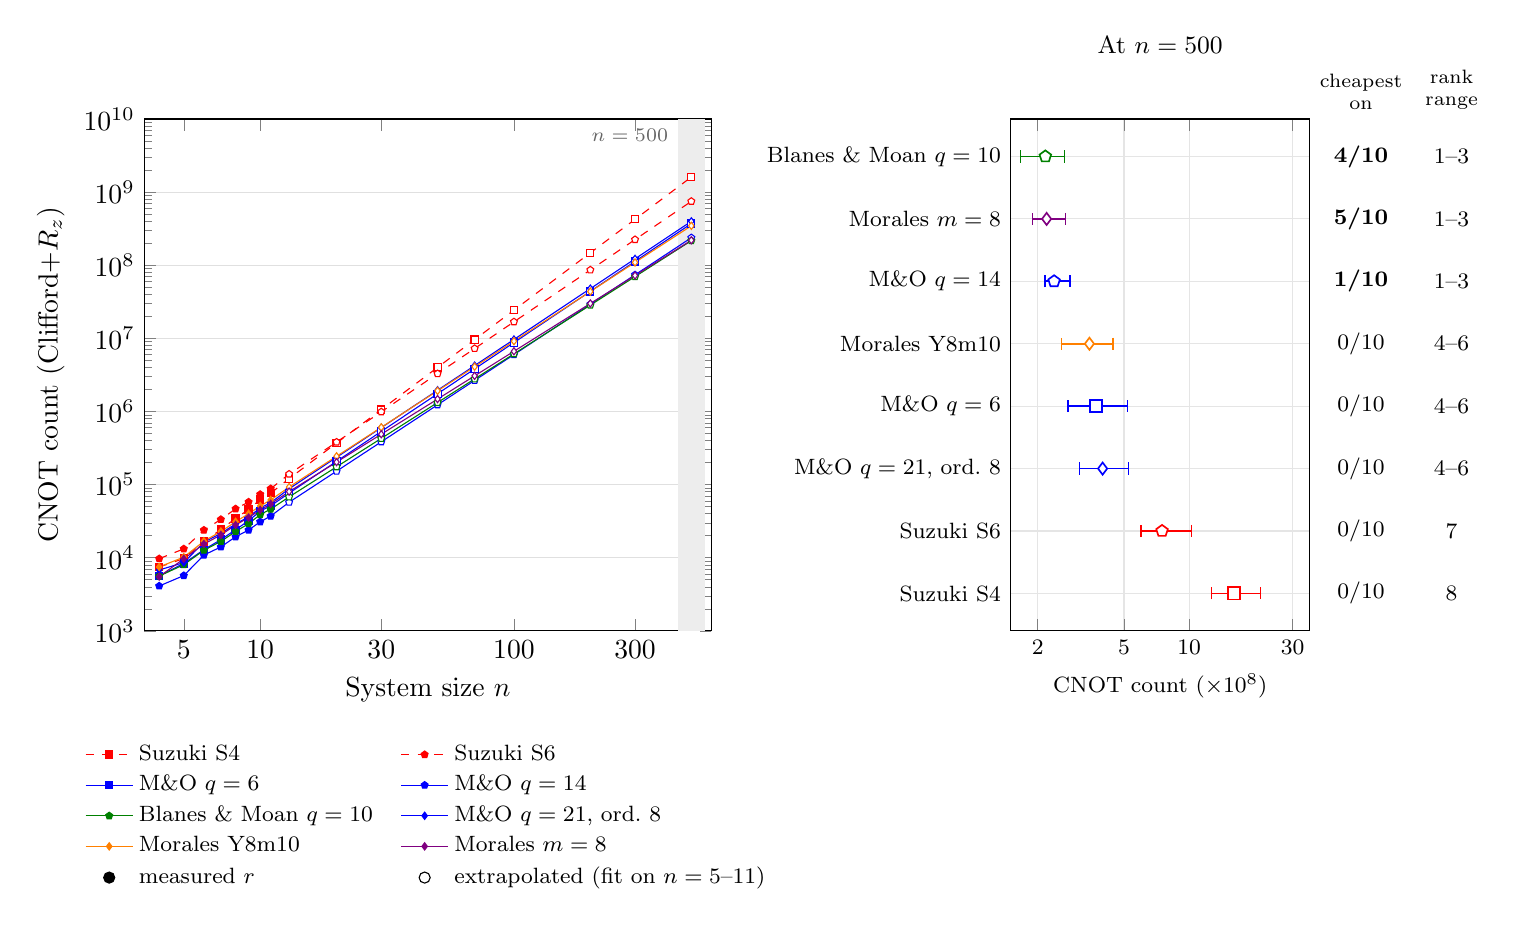
\begin{tikzpicture}
  \begin{loglogaxis}[
    name=main, scale only axis,
    width=7.2cm, height=6.5cm,
    xlabel={System size $n$},
    ylabel={CNOT count (Clifford+$R_z$)},
    xtick={5,10,30,100,300}, xticklabels={5,10,30,100,300},
    xmin=3.5, xmax=600, ymin=1000, ymax=1e+10,
    ymajorgrids=true, grid style={black!12},
    legend style={at={(0.5,-0.2)}, anchor=north, draw=none, font=\footnotesize,
      legend columns=2, /tikz/every even column/.append style={column sep=8pt}},
    legend cell align=left,
  ]
    \fill[black!7] (axis cs:442.478,1000) rectangle (axis cs:565,1e+10);
    \node[anchor=north east, font=\scriptsize, black!60] at (axis cs:442.478,1e+10) {$n=500$};
    % suzuki4: measured n, mean over seeds, bars min..max over seeds
    \addplot[red, dashed, mark=square*, mark size=1.3pt, mark options={solid, fill=red}] coordinates {
      (4,7459.2)
      (5,9744)
      (6,16707.6)
      (7,24284.4)
      (8,34540.8)
      (9,45549)
      (10,62412)
      (11,76230)
    };
    \addlegendentry{Suzuki S4}
    % suzuki4: extrapolated, r = ceil(3.65267 n^1.59931), per step = 42 n + 0; bars min..max of per-seed fits
    \addplot[red, dashed, mark=square*, mark size=1.3pt, mark options={solid, fill=white}, mark indices={2,...,10}, forget plot] coordinates {
      (11,76230)
      (13,120830)
      (20,370020)
      (30,1.06155e+06)
      (50,4.00848e+06)
      (70,9.61968e+06)
      (100,2.43394e+07)
      (200,1.47922e+08)
      (300,4.25239e+08)
      (500,1.60899e+09)
    };
    % suzuki6: measured n, mean over seeds, bars min..max over seeds
    \addplot[red, dashed, mark=pentagon*, mark size=1.3pt, mark options={solid, fill=red}] coordinates {
      (4,9696)
      (5,13231)
      (6,23876.4)
      (7,33370.4)
      (8,46702.4)
      (9,57812.4)
      (10,73528)
      (11,87991.2)
    };
    \addlegendentry{Suzuki S6}
    % suzuki6: extrapolated, r = ceil(1.63295 n^1.35284), per step = 202 n + 0; bars min..max of per-seed fits
    \addplot[red, dashed, mark=pentagon*, mark size=1.3pt, mark options={solid, fill=white}, mark indices={2,...,10}, forget plot] coordinates {
      (11,87991.2)
      (13,139178)
      (20,381780)
      (30,989598)
      (50,3.2926e+06)
      (70,7.26796e+06)
      (100,1.68428e+07)
      (200,8.62823e+07)
      (300,2.24481e+08)
      (500,7.49087e+08)
    };
    % mo-q6: measured n, mean over seeds, bars min..max over seeds
    \addplot[blue, solid, mark=square*, mark size=1.3pt, mark options={solid, fill=blue}] coordinates {
      (4,5660)
      (5,8350)
      (6,12870)
      (7,17675)
      (8,24160)
      (9,32085)
      (10,43300)
      (11,51260)
    };
    \addlegendentry{M\&O $q=6$}
    % mo-q6: extrapolated, r = ceil(3.93927 n^1.32338), per step = 50 n + 0; bars min..max of per-seed fits
    \addplot[blue, solid, mark=square*, mark size=1.3pt, mark options={solid, fill=white}, mark indices={2,...,10}, forget plot] coordinates {
      (11,51260)
      (13,76505)
      (20,207900)
      (30,533100)
      (50,1.74725e+06)
      (70,3.82165e+06)
      (100,8.761e+06)
      (200,4.3965e+07)
      (300,1.13001e+08)
      (500,3.71342e+08)
    };
    % mo-q14: measured n, mean over seeds, bars min..max over seeds
    \addplot[blue, solid, mark=pentagon*, mark size=1.3pt, mark options={solid, fill=blue}] coordinates {
      (4,4104)
      (5,5700)
      (6,10875.6)
      (7,14044.8)
      (8,19334.4)
      (9,23905.8)
      (10,31008)
      (11,37118.4)
    };
    \addlegendentry{M\&O $q=14$}
    % mo-q14: extrapolated, r = ceil(1.412 n^1.28559), per step = 114 n + 0; bars min..max of per-seed fits
    \addplot[blue, solid, mark=pentagon*, mark size=1.3pt, mark options={solid, fill=white}, mark indices={2,...,10}, forget plot] coordinates {
      (11,37118.4)
      (13,57353.4)
      (20,152760)
      (30,384750)
      (50,1.23348e+06)
      (70,2.65973e+06)
      (100,6.00438e+06)
      (200,2.92889e+07)
      (300,7.40054e+07)
      (500,2.37981e+08)
    };
    % bm-q10: measured n, mean over seeds, bars min..max over seeds
    \addplot[green!50!black, solid, mark=pentagon*, mark size=1.3pt, mark options={solid, fill=green!50!black}] coordinates {
      (4,5608.8)
      (5,8036)
      (6,12644.4)
      (7,16703.4)
      (8,22828.8)
      (9,29151)
      (10,38868)
      (11,46182.4)
    };
    \addlegendentry{Blanes \& Moan $q=10$}
    % bm-q10: extrapolated, r = ceil(2.82314 n^1.2111), per step = 82 n + 0; bars min..max of per-seed fits
    \addplot[green!50!black, solid, mark=pentagon*, mark size=1.3pt, mark options={solid, fill=white}, mark indices={2,...,10}, forget plot] coordinates {
      (11,46182.4)
      (13,67904.2)
      (20,175152)
      (30,428532)
      (50,1.32553e+06)
      (70,2.78964e+06)
      (100,6.1418e+06)
      (200,2.84934e+07)
      (300,6.99427e+07)
      (500,2.16874e+08)
    };
    % mo-o8-q21: measured n, mean over seeds, bars min..max over seeds
    \addplot[blue, solid, mark=diamond*, mark size=1.3pt, mark options={solid, fill=blue}] coordinates {
      (4,6800)
      (5,8585)
      (6,16320)
      (7,21539)
      (8,28968)
      (9,36261)
      (10,47770)
      (11,56661)
    };
    \addlegendentry{M\&O $q=21$, ord.~8}
    % mo-o8-q21: extrapolated, r = ceil(1.3736 n^1.30758), per step = 170 n + 0; bars min..max of per-seed fits
    \addplot[blue, solid, mark=diamond*, mark size=1.3pt, mark options={solid, fill=white}, mark indices={2,...,10}, forget plot] coordinates {
      (11,56661)
      (13,87737)
      (20,236300)
      (30,601290)
      (50,1.95245e+06)
      (70,4.24235e+06)
      (100,9.6662e+06)
      (200,4.79366e+07)
      (300,1.22364e+08)
      (500,3.98548e+08)
    };
    % morales-y8m10: measured n, mean over seeds, bars min..max over seeds
    \addplot[orange, solid, mark=diamond*, mark size=1.3pt, mark options={solid, fill=orange}] coordinates {
      (4,7480)
      (5,10200)
      (6,16830)
      (7,22848)
      (8,31008)
      (9,39933)
      (10,51000)
      (11,61710)
    };
    \addlegendentry{Morales Y8m10}
    % morales-y8m10: extrapolated, r = ceil(1.66328 n^1.25438), per step = 170 n + 0; bars min..max of per-seed fits
    \addplot[orange, solid, mark=diamond*, mark size=1.3pt, mark options={solid, fill=white}, mark indices={2,...,10}, forget plot] coordinates {
      (11,61710)
      (13,92599)
      (20,244120)
      (30,607410)
      (50,1.9176e+06)
      (70,4.09836e+06)
      (100,9.1596e+06)
      (200,4.3758e+07)
      (300,1.09303e+08)
      (500,3.46477e+08)
    };
    % morales-m8: measured n, mean over seeds, bars min..max over seeds
    \addplot[violet, solid, mark=diamond*, mark size=1.3pt, mark options={solid, fill=violet}] coordinates {
      (4,5520)
      (5,9660)
      (6,15400.8)
      (7,20479.2)
      (8,28041.6)
      (9,35397)
      (10,44988)
      (11,54496.2)
    };
    \addlegendentry{Morales $m=8$}
    % morales-m8: extrapolated, r = ceil(2.19247 n^1.17079), per step = 138 n + 0; bars min..max of per-seed fits
    \addplot[violet, solid, mark=diamond*, mark size=1.3pt, mark options={solid, fill=white}, mark indices={2,...,10}, forget plot] coordinates {
      (11,54496.2)
      (13,80191.8)
      (20,203136)
      (30,488934)
      (50,1.47936e+06)
      (70,3.07188e+06)
      (100,6.66264e+06)
      (200,3.0026e+07)
      (300,7.24417e+07)
      (500,2.19834e+08)
    };
    \addlegendimage{only marks, black, mark=*, mark options={solid, fill=black}}
    \addlegendentry{measured $r$}
    \addlegendimage{only marks, black, mark=*, mark options={solid, fill=white}}
    \addlegendentry{extrapolated (fit on $n = 5$--$11$)}
  \end{loglogaxis}
  \begin{semilogxaxis}[
    scale only axis, clip=false,
    at={(11.0cm,0cm)}, anchor=south west,
    width=3.8cm, height=6.5cm,
    title={At $n = 500$}, title style={font=\small, yshift=14pt},
    xlabel={CNOT count ($\times 10^{8}$)}, xlabel style={font=\footnotesize},
    xmin=1.5e+08, xmax=3.6e+09, xtick={2e+08,5e+08,1e+09,3e+09}, xticklabels={2,5,10,30},
    xminorticks=false,
    y dir=reverse, ymin=0.4, ymax=8.6, ytick={1,2,3,4,5,6,7,8},
    yticklabels={{Blanes \& Moan $q=10$},{Morales $m=8$},{M\&O $q=14$},{Morales Y8m10},{M\&O $q=6$},{M\&O $q=21$, ord.~8},{Suzuki S6},{Suzuki S4}},
    tick label style={font=\footnotesize}, ytick style={draw=none},
    xmajorgrids=true, ymajorgrids=true, grid style={black!10},
  ]
    % bm-q10: plotted 2.16874e+08, seeds 1.65886e+08..2.65106e+08, cheapest on 4/10, rank 1..3
    \addplot[green!50!black, only marks, mark=pentagon*, mark size=2.2pt, mark options={solid, fill=white, line width=0.6pt}, error bars/.cd, x dir=both, x explicit, error bar style={solid, line width=0.6pt}] coordinates {
      (2.16874e+08,1) += (4.82324e+07,0) -= (5.09876e+07,0)
    };
    % morales-m8: plotted 2.19834e+08, seeds 1.89336e+08..2.67651e+08, cheapest on 5/10, rank 1..3
    \addplot[violet, only marks, mark=diamond*, mark size=2.2pt, mark options={solid, fill=white, line width=0.6pt}, error bars/.cd, x dir=both, x explicit, error bar style={solid, line width=0.6pt}] coordinates {
      (2.19834e+08,2) += (4.7817e+07,0) -= (3.0498e+07,0)
    };
    % mo-q14: plotted 2.37981e+08, seeds 2.16201e+08..2.82036e+08, cheapest on 1/10, rank 1..3
    \addplot[blue, only marks, mark=pentagon*, mark size=2.2pt, mark options={solid, fill=white, line width=0.6pt}, error bars/.cd, x dir=both, x explicit, error bar style={solid, line width=0.6pt}] coordinates {
      (2.37981e+08,3) += (4.40553e+07,0) -= (2.17797e+07,0)
    };
    % morales-y8m10: plotted 3.46477e+08, seeds 2.56615e+08..4.4489e+08, cheapest on 0/10, rank 4..6
    \addplot[orange, only marks, mark=diamond*, mark size=2.2pt, mark options={solid, fill=white, line width=0.6pt}, error bars/.cd, x dir=both, x explicit, error bar style={solid, line width=0.6pt}] coordinates {
      (3.46477e+08,4) += (9.8413e+07,0) -= (8.9862e+07,0)
    };
    % mo-q6: plotted 3.71342e+08, seeds 2.758e+08..5.21575e+08, cheapest on 0/10, rank 4..6
    \addplot[blue, only marks, mark=square*, mark size=2.2pt, mark options={solid, fill=white, line width=0.6pt}, error bars/.cd, x dir=both, x explicit, error bar style={solid, line width=0.6pt}] coordinates {
      (3.71342e+08,5) += (1.50232e+08,0) -= (9.55425e+07,0)
    };
    % mo-o8-q21: plotted 3.98548e+08, seeds 3.12715e+08..5.27085e+08, cheapest on 0/10, rank 4..6
    \addplot[blue, only marks, mark=diamond*, mark size=2.2pt, mark options={solid, fill=white, line width=0.6pt}, error bars/.cd, x dir=both, x explicit, error bar style={solid, line width=0.6pt}] coordinates {
      (3.98548e+08,6) += (1.28537e+08,0) -= (8.5833e+07,0)
    };
    % suzuki6: plotted 7.49087e+08, seeds 5.98829e+08..1.02475e+09, cheapest on 0/10, rank 7..7
    \addplot[red, only marks, mark=pentagon*, mark size=2.2pt, mark options={solid, fill=white, line width=0.6pt}, error bars/.cd, x dir=both, x explicit, error bar style={solid, line width=0.6pt}] coordinates {
      (7.49087e+08,7) += (2.75659e+08,0) -= (1.50258e+08,0)
    };
    % suzuki4: plotted 1.60899e+09, seeds 1.26284e+09..2.13375e+09, cheapest on 0/10, rank 8..8
    \addplot[red, only marks, mark=square*, mark size=2.2pt, mark options={solid, fill=white, line width=0.6pt}, error bars/.cd, x dir=both, x explicit, error bar style={solid, line width=0.6pt}] coordinates {
      (1.60899e+09,8) += (5.24758e+08,0) -= (3.46154e+08,0)
    };
    \node[anchor=south, font=\scriptsize, align=center] at ([xshift=0.65cm]axis cs:3.6e+09,0.4) {cheapest\\on};
    \node[anchor=south, font=\scriptsize, align=center] at ([xshift=1.8cm]axis cs:3.6e+09,0.4) {rank\\range};
    \node[font=\footnotesize\bfseries] at ([xshift=0.65cm]axis cs:3.6e+09,1) {4/10};
    \node[font=\footnotesize] at ([xshift=1.8cm]axis cs:3.6e+09,1) {1--3};
    \node[font=\footnotesize\bfseries] at ([xshift=0.65cm]axis cs:3.6e+09,2) {5/10};
    \node[font=\footnotesize] at ([xshift=1.8cm]axis cs:3.6e+09,2) {1--3};
    \node[font=\footnotesize\bfseries] at ([xshift=0.65cm]axis cs:3.6e+09,3) {1/10};
    \node[font=\footnotesize] at ([xshift=1.8cm]axis cs:3.6e+09,3) {1--3};
    \node[font=\footnotesize] at ([xshift=0.65cm]axis cs:3.6e+09,4) {0/10};
    \node[font=\footnotesize] at ([xshift=1.8cm]axis cs:3.6e+09,4) {4--6};
    \node[font=\footnotesize] at ([xshift=0.65cm]axis cs:3.6e+09,5) {0/10};
    \node[font=\footnotesize] at ([xshift=1.8cm]axis cs:3.6e+09,5) {4--6};
    \node[font=\footnotesize] at ([xshift=0.65cm]axis cs:3.6e+09,6) {0/10};
    \node[font=\footnotesize] at ([xshift=1.8cm]axis cs:3.6e+09,6) {4--6};
    \node[font=\footnotesize] at ([xshift=0.65cm]axis cs:3.6e+09,7) {0/10};
    \node[font=\footnotesize] at ([xshift=1.8cm]axis cs:3.6e+09,7) {7};
    \node[font=\footnotesize] at ([xshift=0.65cm]axis cs:3.6e+09,8) {0/10};
    \node[font=\footnotesize] at ([xshift=1.8cm]axis cs:3.6e+09,8) {8};
  \end{semilogxaxis}
\end{tikzpicture}
